\subsection{Serviços Web}\label{2-fundamentacao-dbs-servicos-web}

Serviços web representam uma solução tecnológica concreta para o desenvolvimento baseado em serviços. Um serviço web utiliza um conjunto de padrões abertos da web para o seu desenvolvimento e invocação (utilização), sendo identificado univocamente por um \textit{Uniform Resource Identifier} (URI). Serviços web são atualmente desenvolvidos de acordo com duas principais abordagens: serviços SOAP e serviços RESTful.

\subsubsection{Serviços SOAP}\label{2-fundamentacao-dbs-servicos-web-soap}

Serviços web SOAP são implementados utilizando um conjunto de tecnologias e padrões abertos de desenvolvimento providos pela W3C~\cite{DACONTA-OBRST-SMITH-2003-The-Semantic-Web}. Os três principais padrões usados no desenvolvimento de serviços web SOAP são o protocolo \textit{Simple Object Access Protocol} (SOAP)~\cite{W3C-2007-SOAP}, a linguagem de descrição de serviços \textit{Web Service Description Language} (WSDL)~\cite{W3C-2007-WSDL} e o registro de serviços \textit{Universal Description Discovery and Integration} (UDDI)~\cite{OASIS-2004-UDDI}.

Interações entre um serviço web SOAP e um cliente de serviço ocorrem com a utilização do protocolo SOAP~\cite{W3C-2007-SOAP}. O protocolo SOAP serializa os dados (objetos) envolvidos em uma interação usando XML. A transferência desses objetos, contidos nas mensagens de requisições, por parte de um cliente, e de respostas, por parte de um provedor, é normalmente realizada por meio do protocolo \textit{Hypertext Transfer Protocol} (HTTP).

A informação contida em uma mensagem criada a partir dos objetos serializados é armazenada no elemento \textit{envelope}, o qual é formado por dois outros elementos: \textit{header} e \textit{body}. O elemento \textit{envelope} define o documento XML como uma mensagem SOAP. O elemento \textit{header} contém informações específicas da mensagem SOAP, como, por exemplo, o endereço de IP de origem. Apesar de ser opcional, o elemento \textit{header}, se presente, deve ser o primeiro elemento-filho de envelope. O elemento \textit{body} armazena as informações referentes à requisição, como o nome dos métodos e o objeto serializado que será enviado na comunicação.

A linguagem WSDL é utilizada para descrever as funcionalidades e a localização de um serviço web SOAP~\cite{W3C-2007-WSDL}. O desenvolvimento de uma especificação WSDL possibilita que um serviço web seja consumido por outras aplicações por meio da disponibilização da descrição dos métodos do serviço, dos seus parâmetros e dos seus valores de retorno. Informações adicionais sobre a linguagem WSDL podem ser encontradas na seção \ref{2-fundamentacao-dbs-servicos-web-descricao-servico-web} deste documento.

UDDI consiste de um padrão para o registro (publicação) e a busca (descoberta) de descrições de serviços web SOAP em um repositório da Internet~\cite{PAPAZOGLOU-GEORGAKOPOULOS-2003-Service-Oriented-Computing, OASIS-2004-UDDI}. A partir do registro UDDI de um serviço web, realizado por um provedor de serviços, um cliente de serviços pode pesquisar e descobrir este serviço web. Além de contribuir com a busca de serviços web a partir de suas descrições, o UDDI provê informações necessárias para que um serviço possa ser reutilizado por um cliente~\cite{OASIS-2004-UDDI}, tais como informações sobre a organização que desenvolveu o serviço web ou sobre as regras de negócio associadas.

Um registro UDDI é criado com base em alguns elementos de uma especificação WSDL. UDDI contém todos os metadados de um serviço web, incluindo uma referência para a descrição WSDL de um serviço e um conjunto de definições que habilita a invocação deste serviço. Um registro UDDI fornece uma interface única (padronizada) que facilita a classificação, a localização, a invocação e o gerenciamento de metadados de um serviço.

%Tais recursos facilitam, portanto, a reutilização de um serviço web e, consequentemente, o desenvolvimento baseado em serviços.

A \figurename~\ref{fig:soap} ilustra a utilização dos diferentes padrões no desenvolvimento e invocação de um serviço web SOAP. A seta pontilhada representa a publicação de uma descrição de serviço WSDL em um repositório UDDI, feita por um provedor de serviços. A seta tracejada representa a descoberta de um serviço web junto a um repositório UDDI feita por um cliente de serviço. Finalmente, a seta sólida representa a requisição de serviço SOAP realizada por um cliente de serviço.

%A seta tracejada e pontilhada, localizada no canto inferior da figura, entre o provedor de serviços e as descrições WSDL, representa uma publicação de descrições de serviço (WSDL) em um repositório UDDI, feita por um provedor de serviços. A seta tracejada, localizada  no canto direito da figura, entre o cliente de serviços e as descrições WSDL, representa uma descoberta de serviços web, por meio de descrições WSDL existentes em um repositório UDDI, feita por um cliente de serviços. A seta sólida, localizada no centro da figura, entre o cliente de serviços e o provedor de serviços, representa uma requisição SOAP, realizada por um cliente de serviços. Por fim, a seta pontilhada, localizada no centro da figura, entre o provedor de serviço e o cliente de serviços, representa uma resposta SOAP para a requisição antes realizada.

%O processo inicia-se com um provedor de serviço desenvolvendo um serviço web e publicando (registrando) este serviço em um repositório UDDI (caixa rosa no centro inferior da figura). Um provedor de serviço pode desenvolver e publicar diversos serviços. Por isso, podemos visualizar diversos serviços (caixas amarelas) dentro do provedor de serviço (caixa cinza, no canto inferior esquerdo da figura). No repositório UDDI, podemos encontrar diversas descrições de serviços que utilizam a linguagem WSDL (caixas verdes, no canto inferior direito da figura). A publicação de descrições de serviço em um repositório UDDI é representada pela seta tracejada e pontilhada (canto inferior da figura, entre o provedor de serviço e as descrições WSDL).

%Ainda conforme a Figura \ref{fig:soap}, o segundo passo é um cliente de serviços (caixa azul, no canto superior direito da figura) realizar a busca e a descoberta de serviços por meio do repositório UDDI. Esta descoberta está representada pela seta tracejada (canto direito da figura, entre o cliente de serviços e as descrições WSDL). O terceiro passo é o cliente de serviços sendo capaz de consumir este serviço (invocar) após a sua descoberta. O consumo é feito por meio de uma requisição SOAP, sendo realizada diretamente no provedor de serviços. Esta requisição SOAP está representada por uma seta sólida (centro da figura, entre o cliente de serviços e o provedor de serviço). Por fim, o serviço retorna uma resposta SOAP para a requisição SOAP ao cliente de serviço. Esta resposta está representada por uma seta pontilhada (centro da figura, entre o provedor de serviço e o cliente de serviços).

\begin{figure}[h]
    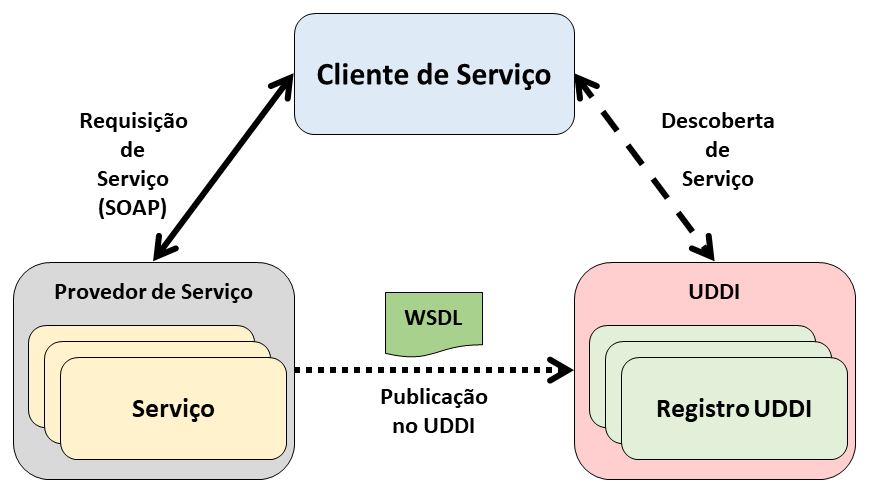
\includegraphics[scale=0.5]{2-fundamentacao-teorica/imagens/arquitetura-orientada-a-servicos(4).png}
    \centering
    \caption[Padrões abertos utilizados em um serviço web SOAP.]{\textbf{Padrões abertos utilizados em um serviço web SOAP.}}
    \label{fig:soap}
\end{figure}

\subsubsection{Serviços RESTful}\label{2-fundamentacao-dbs-servicos-web-restful}

REST (\textit{Representational State Transfer}) foi proposto como um modelo arquitetônico para guiar o projeto de desenvolvimento de sistemas computacionais distribuídos cujas interações entre as diferentes partes deste sistema são realizadas por meio do protocolo HTTP~\cite{FIELDING-2000-REST, CARDOSO-2006-Semantic-Web-Services}. REST é definido a partir de um conjunto de seis restrições arquitetônicas:

\begin{enumerate}

\item
\textit{Arquitetura Cliente-Servidor}, a qual separa a arquitetura de uma aplicação e as responsabilidades em duas partes, fazendo com que o cliente e o provedor não se preocupem com as atividades um do outro;

\item
\textit{Interações sem estado}, as quais definem que toda requisição contenha todas as informações necessárias para que o provedor consiga entendê-la e processá-la, sem a necessidade de informações adicionais ou providas por terceiros;

\item
\textit{Informações em cache}, as quais permitem que recursos muito requisitados por clientes possam ser armazenados, temporariamente, em cache, evitando processamento desnecessário e aumentando significativamente o desempenho;

\item
\textit{Interface uniforme}, a qual define um contrato para a comunicação entre clientes e provedores de serviços. Este contrato apresenta regras usadas para tornar um componente genérico, facilitando sua manutenção e expansão;

\item
\textit{Sistema em camadas}, o qual determina que o sistema seja estruturado em camadas hierárquicas, sendo que cada camada possui uma função específica. Essa estrutura possibilita que responsabilidades possam ser distribuídas entre as camadas, de modo que cada componente do sistema tenha papel e responsabilidades bem definidos;

\item
\textit{Código sob demanda}, o qual, apesar de ser opcional, permite que o cliente possa estender a parte lógica do provedor por meio de \textit{applets} e \textit{scripts}. Isso permite que diferentes clientes possam se comportar de maneiras diferentes, conforme suas necessidades, mesmo que consumam os mesmos serviços disponíveis no provedor.

\end{enumerate}

Os serviços criados com base no modelo arquitetônico REST são chamados de serviços RESTful. Estes serviços não são vinculados a uma tecnologia em particular, ou seja, podem ser desenvolvidos em qualquer plataforma ou linguagem de programação. Os serviços RESTful são mais simples de serem desenvolvidos do que os serviços SOAP, pois não impõem restrições quanto ao formato das mensagens trocadas entre as entidades envolvidas em uma interação. Tal característica permite que o desenvolvedor possa optar por um formato mais adequado para as mensagens do sistema de acordo com sua necessidade. Os formatos de mensagens mais comuns são JSON, XML e texto puro.

%A ausência formal de uma linguagem para descrever os serviços RESTful pode gerar problemas de interoperabilidade entre serviços e clientes. Embora não sejam obrigatórias, especificações da interface de um serviço podem ser criadas usando, por exemplo, a linguagem \textit{Web Application Description Language} (WADL)~\cite{W3C-2009-WADL}.

\subsubsection{Descrição de Serviços Web}\label{2-fundamentacao-dbs-servicos-web-descricao-servico-web}

%\hl{remover referencias de WSDL1.1 e simplificar o texto de WSDL2.0}

A descrição de um serviço web é composta por um conjunto de informações que definem como este serviço pode ser acessado. Tais informações incluem as operações disponíveis, os parâmetros e os valores de retorno, bem como a localização (endereço) do serviço.

Inicialmente, a linguagem \textit{Web Service Description Language} (WSDL) focou na especificação de serviços SOAP (até a versão 1.1 desta linguagem~\cite{W3C-2001-WSDL1.1}). Contudo, WSDL 1.1 não suportava a descrição de um serviço RESTful, pois não provia recursos suficientes para a descrição de todos os métodos HTTP possíveis de serem usados em um serviço RESTful. Assim, a versão 2.0 de WSDL~\cite{W3C-2007-WSDL} foi criada a fim de resolver tais restrições.

Outras abordagens, tais como \textit{Web Application Description Language} (WADL) \cite{W3C-2009-WADL} e \textit{OpenAPI}~\cite{SWAGGER-2017-OpenAPI-Specification}, podem ser utilizadas para a descrição de serviços RESTful. Porém, estas abordagens não são o foco deste trabalho.

%Dentre os problemas existentes, a versão 1.1 provia suporte apenas a serviços SOAP. A versão 2.0 da linguagem WSDL provê total suporte à descrições de serviços RESTful. Com isso, gostaríamos de ressaltar que o foco de interesse deste trabalho é na versão 2.0 do WSDL. Adicionalmente, um serviço RESTful pode ser descrito também por meio de \textit{Web Application Description Language} (WADL)~\cite{W3C-2009-WADL}.

%Atualmente, a especificação WSDL encontra-se na versão 2.0. Esta versão foi criada a fim de resolver problemas existentes de interoperabilidade contidos na versão 1.1. Dentre os problemas existentes, a versão 1.1 provia suporte apenas aos métodos GET e POST do protocolo HTTP. Já a versão 2.0 do WSDL tem total suporte para o protocolo HTTP. Esta versão passou a aceitar todos os métodos de requisições do HTTP – não apenas os métodos GET e POST, como na versão 1.1. Com isso, a descrição de serviços RESTful passou a ser suportada.

%Adicionalmente, WSDL 2.0 tem suporte à \textit{Internationalized Resource Identifiers} (IRIs). IRIs são um conjunto de URIs com suporte extra à internacionalização. Enquanto uma URI suporta apenas um conjunto limitado de caracteres do alfabeto inglês, números europeus e alguns símbolos, uma IRI permite usar caracteres de diversos alfabetos~\cite{W3C-2007-WSDL-Primer}.

%O WSDL 2.0 descreve um serviço da Web em dois estágios fundamentais: um abstrato e um concreto. Dentro de cada estágio, a descrição usa várias construções para promover a reutilização da descrição e separar as preocupações de design independentes.

A linguagem WSDL descreve um serviço web em duas partes fundamentais: parte abstrata e parte concreta. Dentro de cada parte, a descrição WSDL utiliza diferentes elementos que possibilitam a reutilização da descrição e também a separação de modelos independentes. A parte abstrata de uma descrição WSDL contém os elementos \textit{types}, \textit{operation} e \textit{interface}, enquanto que a parte concreta contém os elementos \textit{binding}, \textit{service} e \textit{endpoint}.

%Em um documento WSDL 2.0, há um conjunto simples de definições, composto por seis tipos de elementos: \textit{types}, \textit{operation} e \textit{interface}, que pertencem à parte abstrata da descrição; e \textit{binding}, \textit{service} e \textit{endpoint}, que pertencem à parte concreta da descrição. 

O elemento \textit{types} (\textit{<wsdl:types>}) representa os tipos de dados usados na comunicação. O elemento \textit{operation} (\textit{<wsdl:operation>}) representa uma descrição abstrata de uma ação (operação) suportada por um serviço, ou seja, representa uma funcionalidade suportada pelo serviço web. Adicionalmente, o elemento relaciona parâmetros de entrada (\textit{<wsdl:input>}) e de saída (\textit{<wsdl:output>}).

Operações (\textit{<wsdl:operation}>) são agrupadas por meio do elemento \textit{interface} (\textit{<wsdl:interface>}). Tal agrupamento tem por objetivo obter um formato padronizado para o transporte das mensagens. O elemento \textit{binding} (\textit{<wsdl:binding>}) especifica os detalhes do formato do transporte para uma ou mais interfaces. O elemento \textit{endpoint} (\textit{<wsdl:endpoint>}) associa um endereço de rede a um \textit{binding}. Finalmente, o elemento \textit{service} (\textit{<wsdl:service>}) agrupa os elementos \textit{endpoint}, a fim de implementar uma interface (\textit{<wsdl:interface>}) comum.

Falhas, também chamadas de exceções, consistem de comportamentos não esperados e não tratados no fluxo normal de execução de uma operação de um serviço. A ocorrência de falhas é representada por um elemento do tipo \textit{fault} (\textit{<wsdl:fault>}). O elemento \textit{fault} é especificado diretamente dentro do elemento \textit{interface}, no mesmo nível dos elementos \textit{operation}. Desta forma, uma mensagem de falha pode ser reutilizada por diferente operações. Os elementos \textit{infault} (\textit{<wsdl:infault>}) e \textit{outfault} (\textit{<wsdl:outfault>}) representam instâncias de falhas de entrada e saída, respectivamente, que podem ocorrer dentro de cada operação. Na ocorrência de uma falha, se esta estiver tratada pelo serviço, a mensagem de resposta (\textit{<wsdl:output>}) de uma operação é substituída pela mensagem da falha.

%A especificação WSDL 2.0 também provê um mecanismo genérico para descrever os tipos de operações por meio dos \textit{Message Exchange Patterns} (MEPs)~\cite{W3C-2002-Web-Service-Message-Exchange-Patterns}. Um MEP é um modelo que estabelece um padrão para a troca de mensagens entre serviços SOAP, por meio da definição da ordem em que mensagens referentes a uma mesma operação são trocadas~\cite{NITZSCHE-LESSEN-LEYMAN-2008-Message-Exchange-Patterns}.

%No WSDL 1.1 haviam apenas quatro tipos de operações: \textit{One-way}, que apresenta um \textit{endpoint} que apenas recebe uma mensagem; Request-response, que apresenta um \textit{endpoint} que recebe uma mensagem e envia uma mensagem correspondente; \textit{Solicit-response}, que apresenta um \textit{endpoint} que envia uma mensagem e recebe uma mensagem correspondente; e \textit{Notification}, que apresenta um \textit{endpoint} que apenas envia uma mensagem. Dessa forma, no WSDL 1.1, era necessário mesclar os quatro tipos de operações a fim de obter resultados desejados pelos serviços. Já o WSDL 2.0 provê um mecanismo genérico para descrever os tipos de operações por meio dos \textit{Message Exchange Patterns} (MEPs)~\cite{W3C-2002-Web-Service-Message-Exchange-Patterns}. Um MEP é um modelo que estabelece um padrão para a troca de mensagens entre serviços SOAP, por meio da definição da ordem em que mensagens referentes a uma mesma operação são trocadas~\cite{NITZSCHE-LESSEN-LEYMAN-2008-Message-Exchange-Patterns}.